\section{Resultados e discussões}
\subsection{Pêndulo de Wilberforce}
Neste experimento foi analisado o movimento do Pêndulo de Wilberforce, no qual foi possível observar-se a curiosa dinâmica que define o fenômeno,
em qual períodos de oscilação no eixo longitudinal se alternam com oscilações no eixo rotacional. Aprofundando-se na análise 
do funcionamento do pêndulo, é possível observar que a alternância de oscilações ocorre com uma dinâmica bem estabelecida, 
quando a massa do pêndulo oscila verticalmente, a mola se comprime e alonga, e consequentemente, seu diâmetro aumenta e diminui,
dando uma ligeira torção ao peso. Dessa forma, ocorre a transferência gradativa entre energias potenciais e cinéticas, o que
faz com que os modos de oscilação se alternem gradativamente, resultando em uma relação inversamente proporcional entre as oscilações.

Uma característica muito importante para a dinâmica do pêndulo, é que, para que ocorra a máxima transferência de energia entre os modos
de oscilação é necessário que os mesmos estejam em frequências similares, para entrarem em ressonância, e o ponto de máxima energia potencial
do movimento de um eixo aconteça enquanto a energia cinética do movimento do outro eixo esteja também em seu ponto máximo.

Essa dinâmica de um sistema físico ou eletrônico no qual dois ou mais osciladores que interagem entre si, de tal forma que a oscilação de 
um dos osciladores afeta a oscilação dos outros, é denominada como oscilador acoplado. Este tipo de sistema faz parte da vida cotidiana da maioria da 
população, um exemplo é a maquina de lavar vertical. Uma vez que, como um pêndulo de Wilberforce, ela realiza oscilações no 
eixo rotacional e oscilações no eixo longitudinal. Essa dinâmica de um oscilador acoplado, lhe confere a propriedade de transferência 
gradual de energia entre os modos de oscilação, e dependência da ressonância entre as oscilações para melhor funcionamento do equipamento.
Dessa forma, se a frequência da rotação estiver muito descalibrada, devido ao acumulo de massa em um ponto do cesto da máquina por exemplo,
pode ocasionar em um transferência excessiva de energia para a oscilação longitudinal, o que pode danificar o máquina.

\subsection{Pêndulo de Torção}  

Para analisar o comportamento do pêndulo de torção em diferentes meios, foi medido o tempo necessário para realizar oscilações tanto no 
ar quanto no óleo. Dessas medições, pontuou-se as 5 primeiras oscilações, e ao realizar uma regressão linear, obteve-se uma expressão que corresponde
ao comportamento do pêndulo, tanto no ar quanto no óleo, como é possível observar nas imagens \label{Troçãonoar} e \label{Torçãonoóleo}.
Dessa forma, utilizando as expressões que correspondem ao comportamento do pêndulo em diferentes meios para calcular qual seria o tempo necessário
para se realizar 10 oscilações, temos:

\begin{figure}[H]
	\centering
	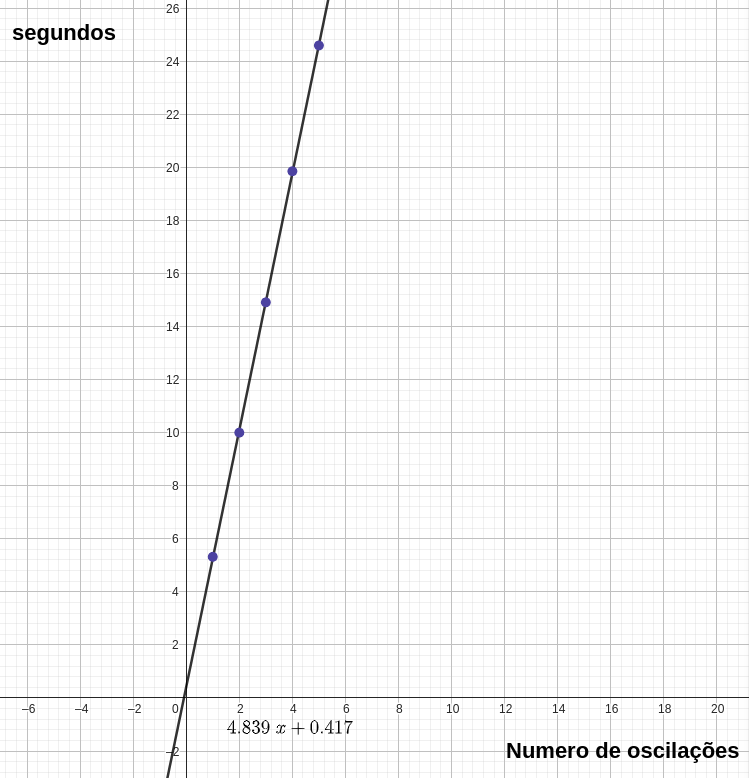
\includegraphics[width=0.35\linewidth]{fig/Torção no ar.png}
	\caption{Gráfico do numero de oscilações do pêndulo de torção no ar por tempo, tendo feita a regressão linear com 5 pontos}
	\label{Torçãonoar}
\end{figure}

\begin{figure}[H]
	\centering
	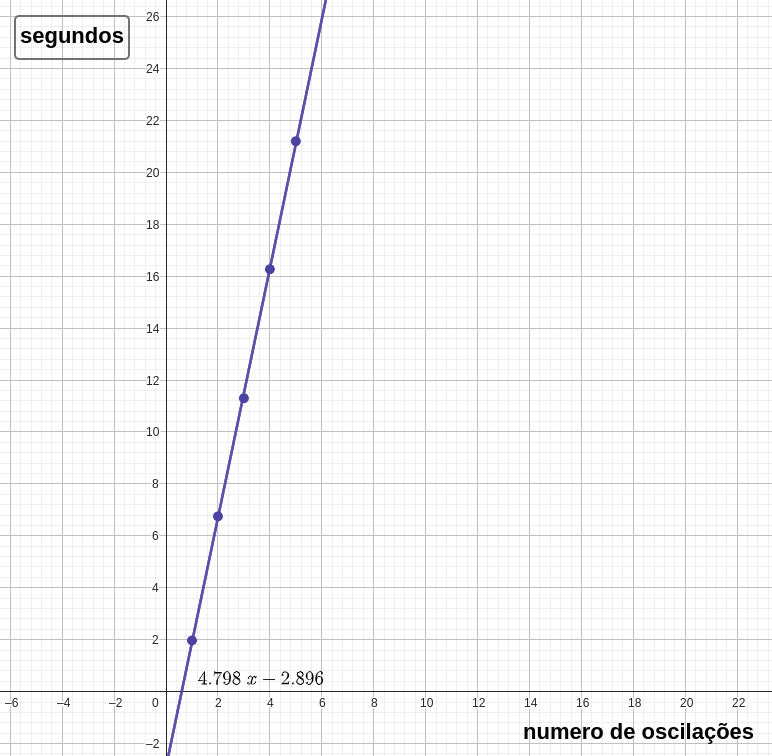
\includegraphics[width=0.35\linewidth]{fig/Oscilações no óleo.png}
	\caption{Gráfico do numero de oscilações do pêndulo de torção no óleo por tempo, tendo feita a regressão linear com 5 pontos}
	\label{Torçãonoóleo}
\end{figure}

Pêndulo no ar:
\begin{align*}
	f(x) &= 4,839x +  0,417 \text{ Sendo "f(x)" o tempo em segundos, e "x" o numero de oscilações} \\
 	f(x) &= 4,839 * 10 + 0,417\\
    f(x) &= \qty{48,807}{s}	
\end{align*}

Pêndulo no óleo:
\begin{align*}
	f(x) &= 4,798x -  2,896 \text{ Sendo "f(x)" o tempo em segundos, e "x" o numero de oscilações}\\
	f(x) &= 4,798 * 10 - 2,896\\
	f(x) &= \qty{45,084}{s}
\end{align*}

\begin{table}[H]
	\caption{Dados obtidos empiricamente do pêndulo de Torção no ar} \label{tabelaar}
	\begin{center}
		\begin{tabular}{c c c}
			\hline
			Oscilação & Tempo (s) & Variação do Tempo (s) \\
			\hline
			1 & 00:05.32 & 00:05.32\\
			2 & 00:10.00 & 00:04.68\\
			3 & 00:14.91 & 00:04.91\\
			4 & 00:19.85 & 00:04.94\\
			5 & 00:24.59 & 00:04.74\\
			6 & 00:29.50 & 00:04.91\\
			7 & 00:34.32 & 00:04.82\\
			8 & 00:39.24 & 00:04.92\\
			9 & 00:44.23 & 00:04.99\\
			10 & 00:48.94 & 00:04.71\\
			\hline
		\end{tabular}
	\end{center}
\end{table}

\begin{table}[H]
	\caption{Dados obtidos empiricamente do pêndulo de Torção no óleo} \label{tabelaóleo}
	\begin{center}
		\begin{tabular}{c c c}
			\hline
			Oscilação & Tempo (s) & Variação do Tempo (s) \\
			\hline
			1 & 00:01.97 & 00:01.97\\
			2 & 00:06.75 & 00:04.78\\
			3 & 00:11.30 & 00:04.55\\
			4 & 00:16.27 & 00:04.97\\
			5 & 00:21.20 & 00:04.93\\
			6 & 00:26.14 & 00:04.94\\
			7 & 00:31.08 & 00:04.94\\
			8 & 00:35.83 & 00:04.75\\
			9 & 00:40.42 & 00:04.59\\
			10 & 00:45.46 & 00:05.04\\
			\hline
		\end{tabular}
	\end{center}
\end{table}

Como observado nas tabelas \ref{tabelaar} e \ref{tabelaóleo}, as previsões da regressão linear estão de acordo com os valores empíricos. Além disso, a análise dos dados permite concluir que, no ar, o pêndulo apresentou oscilações com variações de tempo bastante regulares, com valor médio aproximado de \qty{4,86}{s} por oscilação. Isso sugere que, nesse meio de baixa resistência, o movimento mantém sua periodicidade e conserva energia por mais tempo.

Já no óleo, embora a média das oscilações também tenha se mantido próxima a \qty{4,85}{s}, a primeira oscilação foi significativamente mais curta (\qty{1,97}{s}), o que pode indicar um erro experimental ou falha na cronometragem. Ao desconsiderar essa medida inicial, a média passa para \qty{4,83}{s}, valor mais coerente com o esperado para um sistema amortecido.

Assim, ao excluir a primeira medição, conclui-se que o pêndulo no ar representa um sistema quase conservativo, enquanto o pêndulo no óleo evidencia a ação de um meio viscoso, que dissipa energia com mais intensidade, reduzindo a amplitude das oscilações com o tempo.




